%%%%%%%%%%%%%%%%%%%%%%%%%%%%%%%%%%%%%%%%%%%%%%%%%%%%%%%%%%%%%

\mainmatter
\setcounter{page}{1}

\lectureseries[\course]{\course}

\auth[\lecAuth]{Lecturer: \lecAuth\\ Scribe: \scribe}
\date{November 19, 2009}

\setaddress

% the following hack starts the lecture numbering at 16
\setcounter{lecture}{15}
\setcounter{chapter}{15}

\lecture{Approximate Modeling}

\section{Approximation Review}
So far we have seen that when $\mathcal{S}\in\mathcal{M}$ we get
$$\lim_{N\to\infty}\thetan=\theta_0 \text{ w.p. } 1$$
and we can find expressions for the variance as in \S\ref{sec:varsinm}. When $\mathcal{S}\notin\mathcal{M}$ we can only approximate the parameters as
$$\lim_{N\to\infty}\thetan=\theta^\ast \text{ w.p. } 1$$
In this case we are performing a $2$-norm minimization that works when we have enough data. This was shown in \S\ref{sec:convergence}. We saw in Example \ref{ex:15arx} that if the system is ARMAX and the model is ARX we could compute $\theta^\ast$.

What does $\theta^\ast$ represent though? Chapter 8 of Ljung looks at $\theta^\ast$ from a transfer function point-of-view. We will look at the effect on the transfer functions when using $\theta^\ast$ and no at what $\theta^\ast$ actually is which will give us a qualitative analysis. This will let us know what $\theta^\ast$ tends to look like.

\subsection{Results So Far}
We already know
\begin{itemize}
\item $\lim_{N\to\infty}V_N(\theta,Z^N) = \bar{V}(\theta) = \bar{E}\{\epsilon^2(t,\theta)\}$
\item $\theta^\ast = \argmin{\theta}\bar{V}(\theta)$
\item $\lim_{N\to\infty}\thetan = \theta^\ast \text{ w.p. } 1$
\end{itemize}

\section{Frequency Domain Analysis}
We also know how to relate time domain minimization to frequency domain minimization. The main tool for this is Parceval's Theorem.
\begin{theorem}
$$\bar{E}\{\epsilon^2(t,\theta)\} = \frac{1}{2\pi}\int_{-\pi}^\pi \Phi_\epsilon(\w,\theta)d\w$$
\end{theorem}
This can also be written as
$$R_\eps(\tau) = \bar{E}\{\ett,\epsilon(t-\tau,\T)\} = \frac{1}{2\pi}\int_{-\pi}^\pi R_\eps(\tau)e^{j\w\tau}d\w$$
At $\tau=0$ this becomes
$$R_\eps(0) = \frac{1}{2\pi}\int_{-\pi}^\pi R_\eps(0)d\w$$
This leads to
\begin{align*}
\T^\ast &= \argmin{\T}\bar{V}(\T) = \argmin{\T}\bar{E}\{\est\} \\
&= \argmin{\T}\frac{1}{2\pi}\int_{-\pi}^\pi \Phi_\eps(\w,\T)d\w
\end{align*}

The main idea is to look the $\Phi_\eps(\w,\T)$ to get an interpretation for $\T^\ast$. We are trying to minimize the surface under the curve in Figure \ref{fig:16spec}.

\begin{figure}[ht!]
	\centering
	\includegraphics[width=.3\textwidth]{images/16spec}
	\caption{Spectrum of prediction error.}
	\label{fig:16spec}
\end{figure}

\section{Open Loop Case}
For the system
$$\mathcal{S}: y(t) = \go u(t) + v(t), \qquad v(t) = \ho e(t)$$
The prediction error is then
\begin{align}
\ett &= \hit[y(t)-\go u(t)] \nonumber \\
&= \hit[\go u(t)+\ho e-\gt u(t)] \nonumber \\
\label{eq:16e1}
&= \hit[(\go-\gt)u(t)+v(t)] \\
\label{eq:16e2}
&= \hit [ (\go - \gt) u(t) + (\ho - \hth) e(t) ] + e(t)
\end{align}

\subsection{Looking at (\ref{eq:16e1})}
Recall that
$$x=Fy \Rightarrow \Phi_x(\w)=|F(e^{i\w})|^2\Phi_y(\w)$$
Now, we see that the spectrum of the prediction error is
$$\Phi_\eps(\w,\T) = |H_\T(e^{i\w})|^{-2}[|G_0(e^{i\w})-G_\T(e^{i\w})|^2\Phi_u(\w) + \Phi_v(\w)$$
We can interpret $\T^\ast$ as
$$\T^\ast = \argmin{\T} \frac{1}{2\pi} \int_{-\pi}^\pi \frac{|G_0(e^{i\w})-G_\T(e^{i\w})|^2\Phi_u(\w)+\Phi_v(\w)}{|H_\T(e^{i\w})|^2}$$
There is a trade-off between fitting $\gt$ onto $\go$ that is weighted by the term $\Phi_u(\w)|H_\T(e^{i\w})|^2$. In this case we also have that $|H_\T(e^{i\w})|^2\sim\Phi_v(\w)$. Since there is a weighting term involved any attempts to fit the system increases the amount that the noise filter is fit to the model as well.

\subsection{Looking at (\ref{eq:16e2})}
The spectrum of the prediction error can also be written as
$$\Phi_\eps(\w,\T) = |H_\T(e^{i\w})|^{-2}[|G_0(e^{i\w})-G_\T(e^{i\w})|^2\Phi_u(\w)+|H_0(e^{i\w})-H_\T(e^{i\w})|^2\lambda]+\lambda$$
With this version we can interpret $\T^\ast$ as a trade-off between fitting $\gt$ onto $\go$ with the weighting term
$$\frac{\Phi_u(\w)}{|H_\T(e^{i\w})|^2}$$
and $\hth$ onto $\ho$ with weighting term
$$\frac{\lambda}{|H_\T(e^{i\w})|^2}$$

Note that this analysis applies to arbitrary model structures.

\begin{example}
Using an OE (output error) model we have that the noise filter is $\hth=1$ and the spectrum of the prediction error is
$$\Phi_\eps(\w,\T) = |G_0(e^{i\w})-G_\T(e^{i\w})|^2\Phi_u(\w)$$
Now, $\T^\ast$ is the fit of $\gt$ onto $\go$ with the weighting determined entirely by the spectrum of the input signal, $\Phi_u(\w)$.

Let the real system dynamics have a response as shown in Figure \ref{fig:16oebode}. If we choose to use a second-order model in open-loop with the input $\{u(t)\}$ white noise we see that $\Phi_u(\w)$ is flat. Also, the second-order dynamics will only capture one of the resonant modes. The flat weighting function with the OE model means that we will capture the largest error which corresponds to the largest resonant mode.

We could design the input spectrum to look like Figure \ref{fig:16uspec} to try and capture other low-frequency responses. Note that $\Phi_u(\w)$, the input spectrum, determines the ``fit'' of the model or $\T^\ast$.
$\lozenge$
\end{example}

\begin{figure}[ht!]
	\centering
	\includegraphics[width=.3\textwidth]{images/16oebode}
	\caption{Bode plot for OE model.}
	\label{fig:16oebode}
\end{figure}

\begin{figure}[ht!]
	\centering
	\includegraphics[width=.3\textwidth]{images/16uspec}
	\caption{Possible spectrum for input signal.}
	\label{fig:16uspec}
\end{figure}

\begin{example}
For the same system shown in Figure \ref{fig:16oebode} we will now attempt to model it with an ARX model, where
$$\gt=\frac{B_\T(q)}{A_\T(q)}, \qquad \hth=\frac{1}{A_\T(q)}$$
Again, we choose to use a second-order model in open loop with the input $\{u(t)\}$ white noise. We will see that when $\mathcal{S}\notin\mathcal{M}$ then the approximation result will be different when using different model structures. The spectrum of the prediction error now becomes
\begin{align*}
\Phi_\eps(\w,\T) &= \frac{|G_0(e^{i\w})-G_\T(e^{i\w})|^2\Phi_u(\w)}{|H_\T(e^{i\w})^2} + \frac{|H_0(e^{i\w})-H_\T(e^{i\w})|^2}{|H_\T(e^{i\w})|^2}\lambda \\
&= |G_0(e^{i\w})-G_\T(e^{i\w})|^2\Phi_u(\w)|A_\T(\w)|^2 + \frac{|H_0(e^{i\w})-H_\T(e^{i\w})|^2}{|H_\T(e^{i\w})|^2}\lambda
\end{align*}
What is the shape of $\Phi_u(w)|A_\T(\w)|^2$? Recall that $\Phi_u(\w)$ is flat which means that the spectrum for the $B_\T(q)$ term will also be flat. So, the shape of the input spectrum will become the inverse of the response of $\gt$ because $A_\T(q)$ is in the denominator of $\gt$. See Figure \ref{fig:16inv}.

\begin{figure}[ht!]
	\centering
	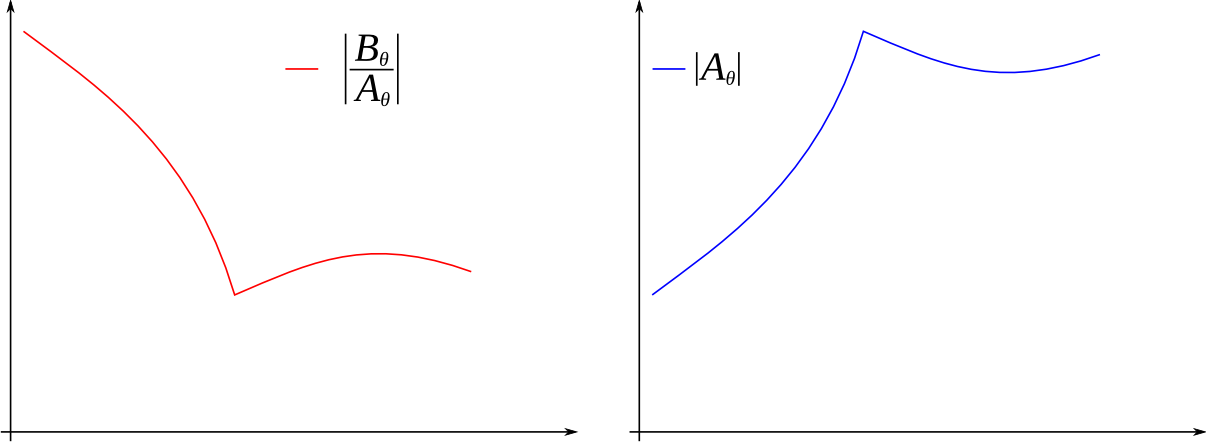
\includegraphics[width=.5\textwidth]{images/16inv}
	\caption{Shape of the filtered input spectrum.}
	\label{fig:16inv}
\end{figure}

This shows that an ARX model has implicit high-frequency weighting because ARX attempts to model the noise and the noise is in the denominator so we get the inverse of the noise model.

Also, note that there still exists a trade-off between fitting $\hth$ onto $\ho$.
$\lozenge$
\end{example}

\section{Design Parameters}
\label{sec:16dp}
How can the engineer influence the model fit when $\mathcal{S}\notin\mathcal{M}$?
\begin{itemize}
\item Change $\Phi_u(\w)$ with experiment design.
\item Change the choice of model structure used.
\item Filter the prediction error.
\end{itemize}
Filtering the prediction error is accomplished by
\begin{align*}
\eps_F(t,\T) &= L(q)\ett \\
\Rightarrow \Phi_{\eps_F}(\w,\T) &= |L(e^{i\w})|^2\Phi_\eps(\w,\T) \\
\Rightarrow \Phi_{\eps_F}(\w) &= |G_0(e^{i\w}) - G_\T(e^{i\w})|^2\frac{\Phi_u(\w)}{|H_\T(e^{i\w})|^2}|L(e^{i\w})|^2 \\
&\qquad + \frac{H_0(e^{i\w}) - H_\T(e^{i\w})|^2}{|H_\T(e^{i\w})|^2}|L(e^{i\w})|^2\lambda
\end{align*}
Keep in mind that $|L(\w)|$ is used to remove spectra, not to amplify it.

\subsection{Another Design Parameter}
The engineer could also choose a model structure and then fix the noise filter to be $H^\ast(q)$, for example instead of $\hth=1$ we could make $H^\ast(q)$ be a band-pass filter. This would give the prediction error as
\begin{align*}
\ett &= \hit[y(t)-\gt u(t)] \\
&= H^{-1\ast}(q,\T)[y(t) - \gt u(t)] \\
&= L(q)[y(t) - \gt u(t)]
\end{align*}
Notice, however, that the term in the braces in the last expression is the prediction error of teh OE model.
$$\Rightarrow \ett = L(q)\eps_{OE}(t,\T)$$
This is the same as the third option in \S\ref{sec:16dp} with $L(q)=H^{-1\ast}(q)$.

\subsection{Filtering the Prediction Error}
In \textsc{Matlab} we can only use \texttt{oe([y u],[nb,nd,nk])} to use the output error model. So how do we apply a filter in \textsc{Matlab}? We use
\begin{align*}
\ett &= \hit[y(t)-\gt u(t)] \\
\Rightarrow L\ett &= \hit[\underbrace{L(q)y(t)}_{y_F} - \gt \underbrace{L(q)u(t)}_{u_F}]
\end{align*}
We just filter the data and call \texttt{oe([yf uf],[nb,nd,nk])}!

\subsection{Closed Loop Case}
This is for the more general case when $u(t)\not\perp e(t)$. We still have the prediction error as
\begin{align*}
\ett &= \hit[y(t)-\gt u(t)] \\
&= \hit[(\go-\gt)u(t)+(\ho-\hth)e(t)]+e(t)
\end{align*}
This gives a spectrum for the prediction error of
\begin{align*}
\Phi_\eps(\w,\T) &= \frac{1}{|H_\T(e^{i\w})|^2}
\left[\begin{array}{c c} (G_0(e^{i\w})-G_\T(e^{i\w})) & (H_0(e^{i\w})-H_\T(e^{i\w})) \end{array}\right] \times \\
&\qquad\times \left[\begin{array}{c c} \Phi_u(\w) & \Phi_{ue}(\w) \\ \Phi_{eu}(\w) & \lambda \end{array}\right]
\left[\begin{array}{c} \overline{G_0(e^{i\w})-G_\T(e^{i\w})} \\ \overline{H_0(e^{i\w})-H_\T(e^{i\w})} \end{array}\right] + \lambda
\end{align*}
Ljung came up with a clever trick using the Schur complement and matrix inversion lemma to rewrite this as
\begin{align*}
\left[\begin{array}{c c} \Phi_u(\w) & \Phi_{ue}(\w) \\ \Phi_{eu}(\w) & \lambda \end{array}\right] &=
\left[\begin{array}{c c} I & 0 \\ \frac{\Phi_{eu}(\w)}{\Phi_u(\w)} & I \end{array}\right]
\left[\begin{array}{c c} \Phi_u(\w) & 0 \\ 0 & \lambda-\frac{|\Phi_{eu}(\w)|^2}{\Phi_u(\w)} \end{array}\right]
\left[\begin{array}{c c} I & \frac{\Phi_{ue}(\w)}{\Phi_u(\w)} \\ 0 & I \end{array}\right]
\end{align*}

We can define a bias term, $B(e^{i\w},\T)$, as
$$B(e^{i\w},\T) = \frac{(H_0(e^{i\w})-H_\T(e^{i\w}))\Phi_{ue}(\w)}{\Phi_u(\w)}$$
Note that the bias term only depends on the noise filter and cross-covariance functions but not on $\go$ or $\gt$. It follows from here that
\begin{align*}
\Phi_\eps(\w,\T) &= \frac{G_0(e^{i\w})+B_\T(e^{i\w})-G_\T(e^{i\w})|^2\Phi_u(\w)}{|H_\T(e^{i\w})|^w} \\
&\qquad + \frac{|H_0(e^{i\w})-H_\T(e^{i\w})|^2}{|H_\T(e^{i\w})|^2}\cdot \left(\lambda-\frac{|\Phi_{ue}(\w)|^2}{\Phi_u(\w)}\right) + \lambda
\end{align*}
There still exists a trade-off between fitting the system (in the first term) and the noise filter (in the second term). Notice that we are also now fitting $\gt$ onto $\go+B_\T(q)$ and not just onto $\go$.

Even if $\mathcal{G}\in\mathcal{M}$ we still get the bias term because we might get the independent parameterization of the system with $\rho_0$ but we still have that $\mathcal{S}\notin\mathcal{M}$ so there does not exist $\theta_0$ such that $H(q,\T_0)=H_0(q)$. The only ways to remove the bias term are to
\begin{itemize}
\item Run open loop experiments so that $\Phi_{ue}(\w)=0$.
\item Make $\hth=\ho$.
\end{itemize}

%%%%%%%%%%%%%%%%%%%%%%%%%%%%%%%%%%%%%%%%%%%%%%%%%%%%%%%%%%%%%